\documentclass[../../Paper.tex]{subfiles}
    
\begin{document}


\begin{table*}[!t]
\centering
\caption{Model fit comparisons of \textit{R. balthica} Temperature Performance Curves}
\label{}
\begin{tabular}{cllllll}
\hline
\multicolumn{1}{l}{Stream Temperature} & \multicolumn{3}{c}{Cubic}             & \multicolumn{3}{c}{Schoolfield}                         \\ \hline
                                       & AIC  & BIC  & R\textasciicircum \{2\} & AIC           & BIC           & R\textasciicircum \{2\} \\ \hline
5.6                                    & -574 & -564 & 0.53                    & \textbf{-584} & \textbf{-576} & \textbf{0.57}           \\
8.1                                    & -305 & -298 & 0.55                    & \textbf{-322} & \textbf{-316} & \textbf{0.66}           \\
9.6                                    & -784 & -773 & 0.58                    & \textbf{-790} & \textbf{-782} & \textbf{0.59}           \\
13.2                                   & -415 & -407 & 0.58                    & \textbf{-424} & \textbf{-418} & \textbf{0.62}           \\
13.9                                   & -421 & -412 & 0.61                    & \textbf{-423} & \textbf{-417} & \textbf{0.61}           \\
14.4                                   & -587 & -577 & 0.58                    & \textbf{-604} & \textbf{-597} & \textbf{0.64}           \\
19.3                                   & -475 & -465 & 0.56                    & \textbf{-483} & \textbf{-476} & \textbf{0.59}           \\ \hline
\end{tabular}
\end{table*}


\subsection*{Data and composition}

The data was collected from the Hengill valley, Southwest Iceland (64\degree03'N: 21\degree18'W) by Dr E. 
O'Gorman, Dr R. Kordas and El\'{e}a Giraud from the Hengill valley between May 2015 to August 2017.
These datasets consisted of a respiration set; respiration data (in micromoles per hour) on
individuals from 7 different streams (5.5 - 19.3 \degree C), exposed to experimental
temperatures ranging from 5-45 \degree C, and a feeding dataset; feeding data (in milligrams per m$^{2}$
per hour) on individuals from 3 different streams (9.6, 14.4 and 19.3 \degree C) exposed to experimental
temperatures ranging from 5.2-27.5 \degree C. Included with both of these datasets was the mass of 
the individuals prior to experimentation; this was used to correct all measured biological traits
by multiplying by $Mass^{\nicefrac{-3}{4}}$. The final datasets consisted of 529 respiration observations, 
and 89 feeding observations. Plots were then run to check for characteristic patterns
in the data, such as a bell curve shape, typical of thermal performance curves (TPCs); following this, several models were run on both datasets using Python 3.6.3 (\cite{van_rossum_python_2001}).

\subsection*{Data modelling}

\begin{figure}[H]
\includegraphics{example_TPC.pdf}
\caption{Example Thermal Performance Curve Plot of \textit{R. balthica}}

\end{figure}

Figure 1 shows a typical temperature performance curve; a near exponential
increase in trait response up to a point (usually referred to as an optimal or peak temperature)
proceeded by a rapid decrease in trait response. Due to the nature of these plots, various models 
have been designed using a range of mathematical equations in an attempt to describe the data, 
with most functions stemming from polynomial models.

Such models include simple phenomenological models (e.g. cubic models) and 
mechanistic models (e.g. Schoolfield model). Both of these methods of modelling 
match observed data with a reasonable amount of accuracy; the difference between 
these two types of models is the underlying theory behind them. 

\subsubsection*{Phenomenological}

Phenomenological models describe the empirical relationship between phenomena,
but do not attempt to explain why the particular variables interact in the way
that they do. The cubic model formulae was as such:

\begin{equation}
B = aT^3 + bT^2 + cT + d
\end{equation}

Where B was the trait of interest (respiration rate), T is the temperature (in 
\degree C) and a,b,c, and d are all mathematical scalars of the function. This 
function was fitted to the entire respiration data set, and also each individual
stream/acclimation temperature.

\subsubsection*{Mechanistic}

A mechanistic models main assumptions are that complex systems can be understood 
by examining its individual parts, and the way in which these phenomena 
interact. 

For this study, a simplified Schoolfield function following from the Metabolic 
Theory of Ecology was used:

\begin{equation}
B = \frac{B_{\theta} e^{\frac{-E}{kT}}}{1 + e^{\frac{E_h}{k} (\frac{1}{T_{pk}} - \frac{1}{T})}}
\end{equation}

Where B is the trait (respiration rate) value, B$_\theta$ is the normalization 
constant, $E$ is the activation energy of the curve (measured in eV)
, $E_h$ is the high temperature deactivation energy of the curve, $T_{pk}$ is the temperature (in K) 
where the model peaks and $k$ is the boltzman constant (8.617 x $10^-5$ eV .$ 
K^{-1}$).

This equation attempts to explain the relationship between temperature, T (in 
Kelvin), and trait, B at a fundamental level. 
Temperature is responsible for driving enzyme chemical reactions, which in turn impact on 
metabolism. B$_\theta$ is the value of the trait at a low temperature 
(10 \degree C), whilst the Arrhenius equation, ($e^{\nicefrac{-E}{kt}}$),
models the temperature dependance of reaction rates during the "normal operating range"
(between 10 - 35 \degree C) (\cite{brown_toward_2004}).Within the Arrhenius equation,  $E$ controls the enzyme activation energy and 
is normally within the range of 0.1 - 1eV, with most studies reporting values between 0.5 - 
0.7, regardless of species or location. $E_h$ controls the high-temperature deactivation energy
of the enzymes, and along with $T_{pk}$, models the rapid descent of the curve. 

The simplified Schoolfield model was used
as low temperature measurements (\textless 5 \degree C) were not made. 


\begin{figure*}[!t]
\centering
\includegraphics{Schoolfield_plots.pdf}
\caption{Schoolfield Temperature performance curves of \textit{R. balthica} plotted for increasing 
acclimation temperatures. Parameters of the function are displayed in each 
unique plot}
\end{figure*}

\begin{figure*}[!t]
\centering
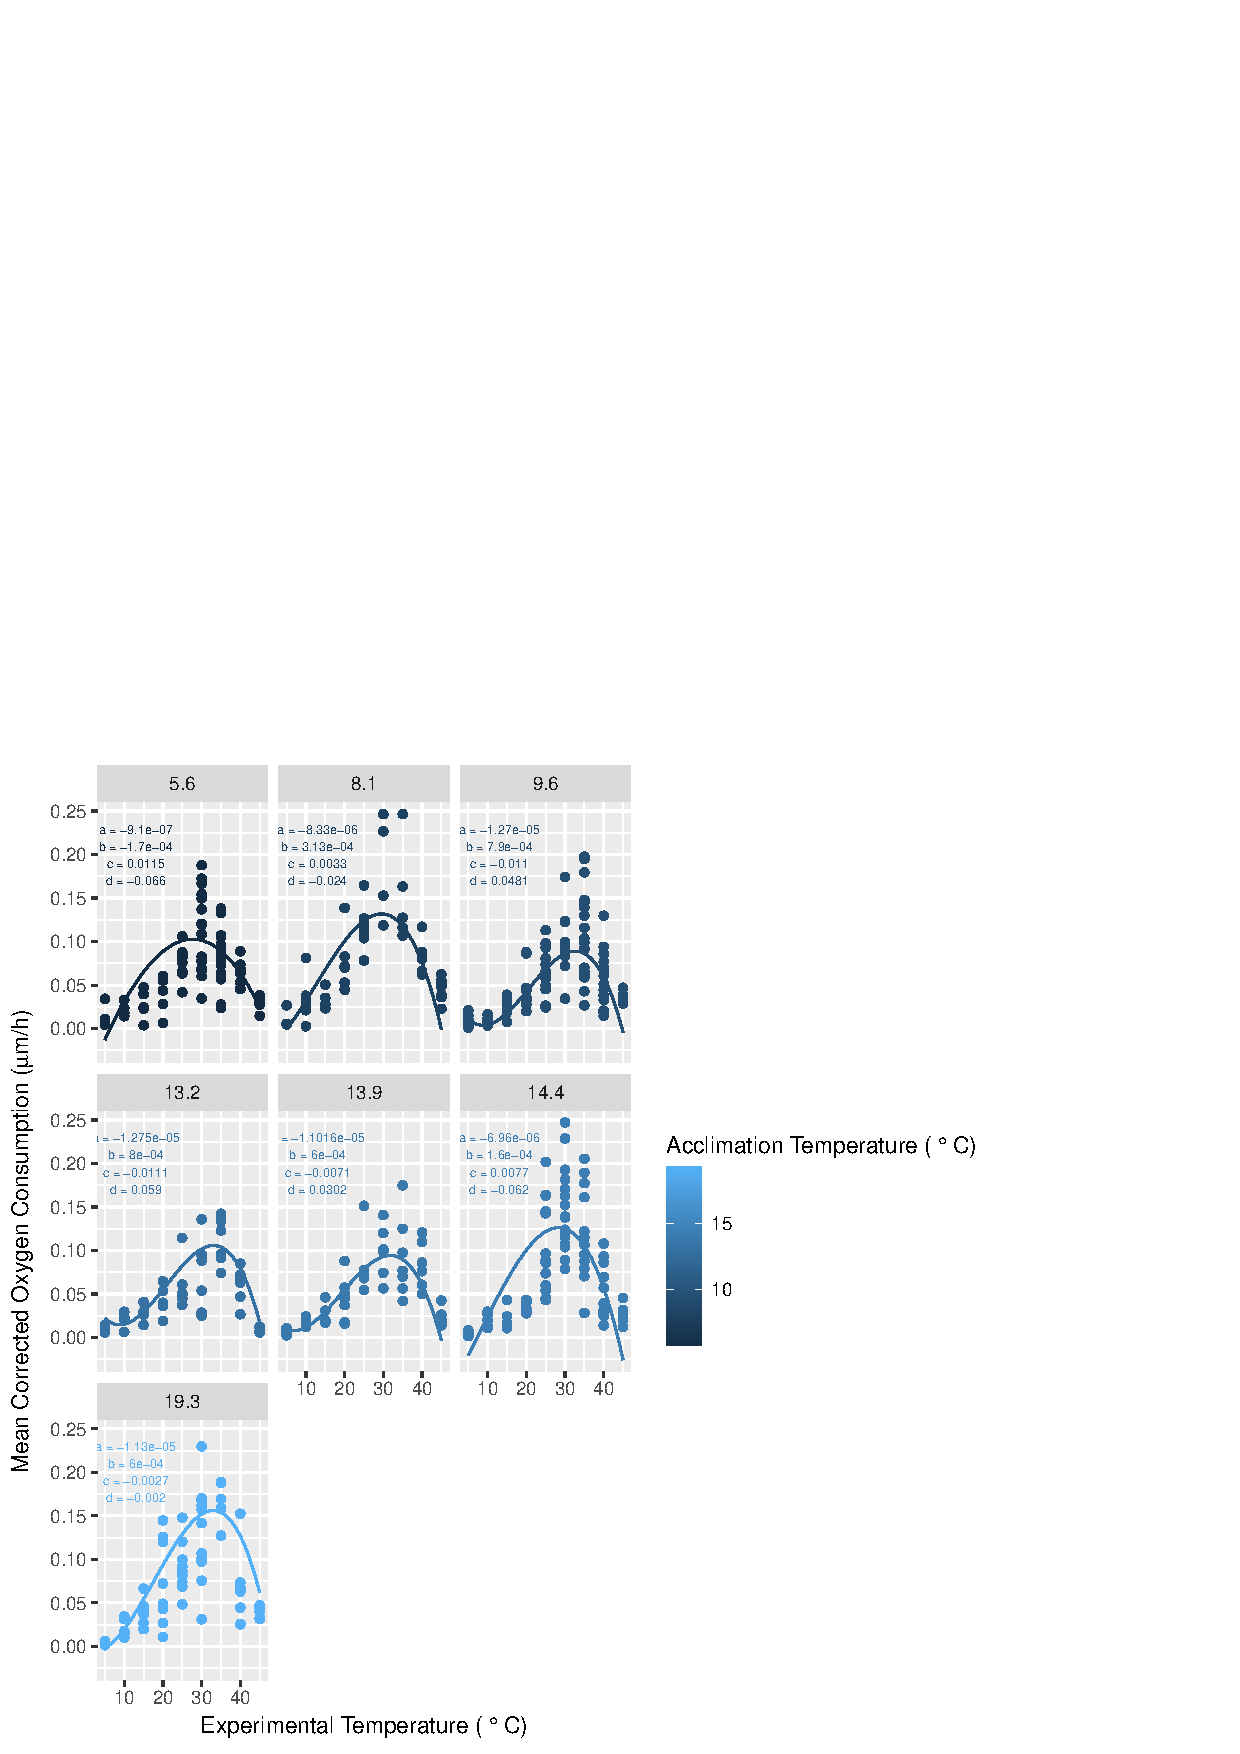
\includegraphics{cubic_plots.pdf}
\caption{Cubic Temperature performance curves of \textit{R. balthica} plotted for increasing 
acclimation temperatures. Parameters of the function are displayed in each 
unique plot}
\end{figure*}

\begin{figure*}[!b]

\centering
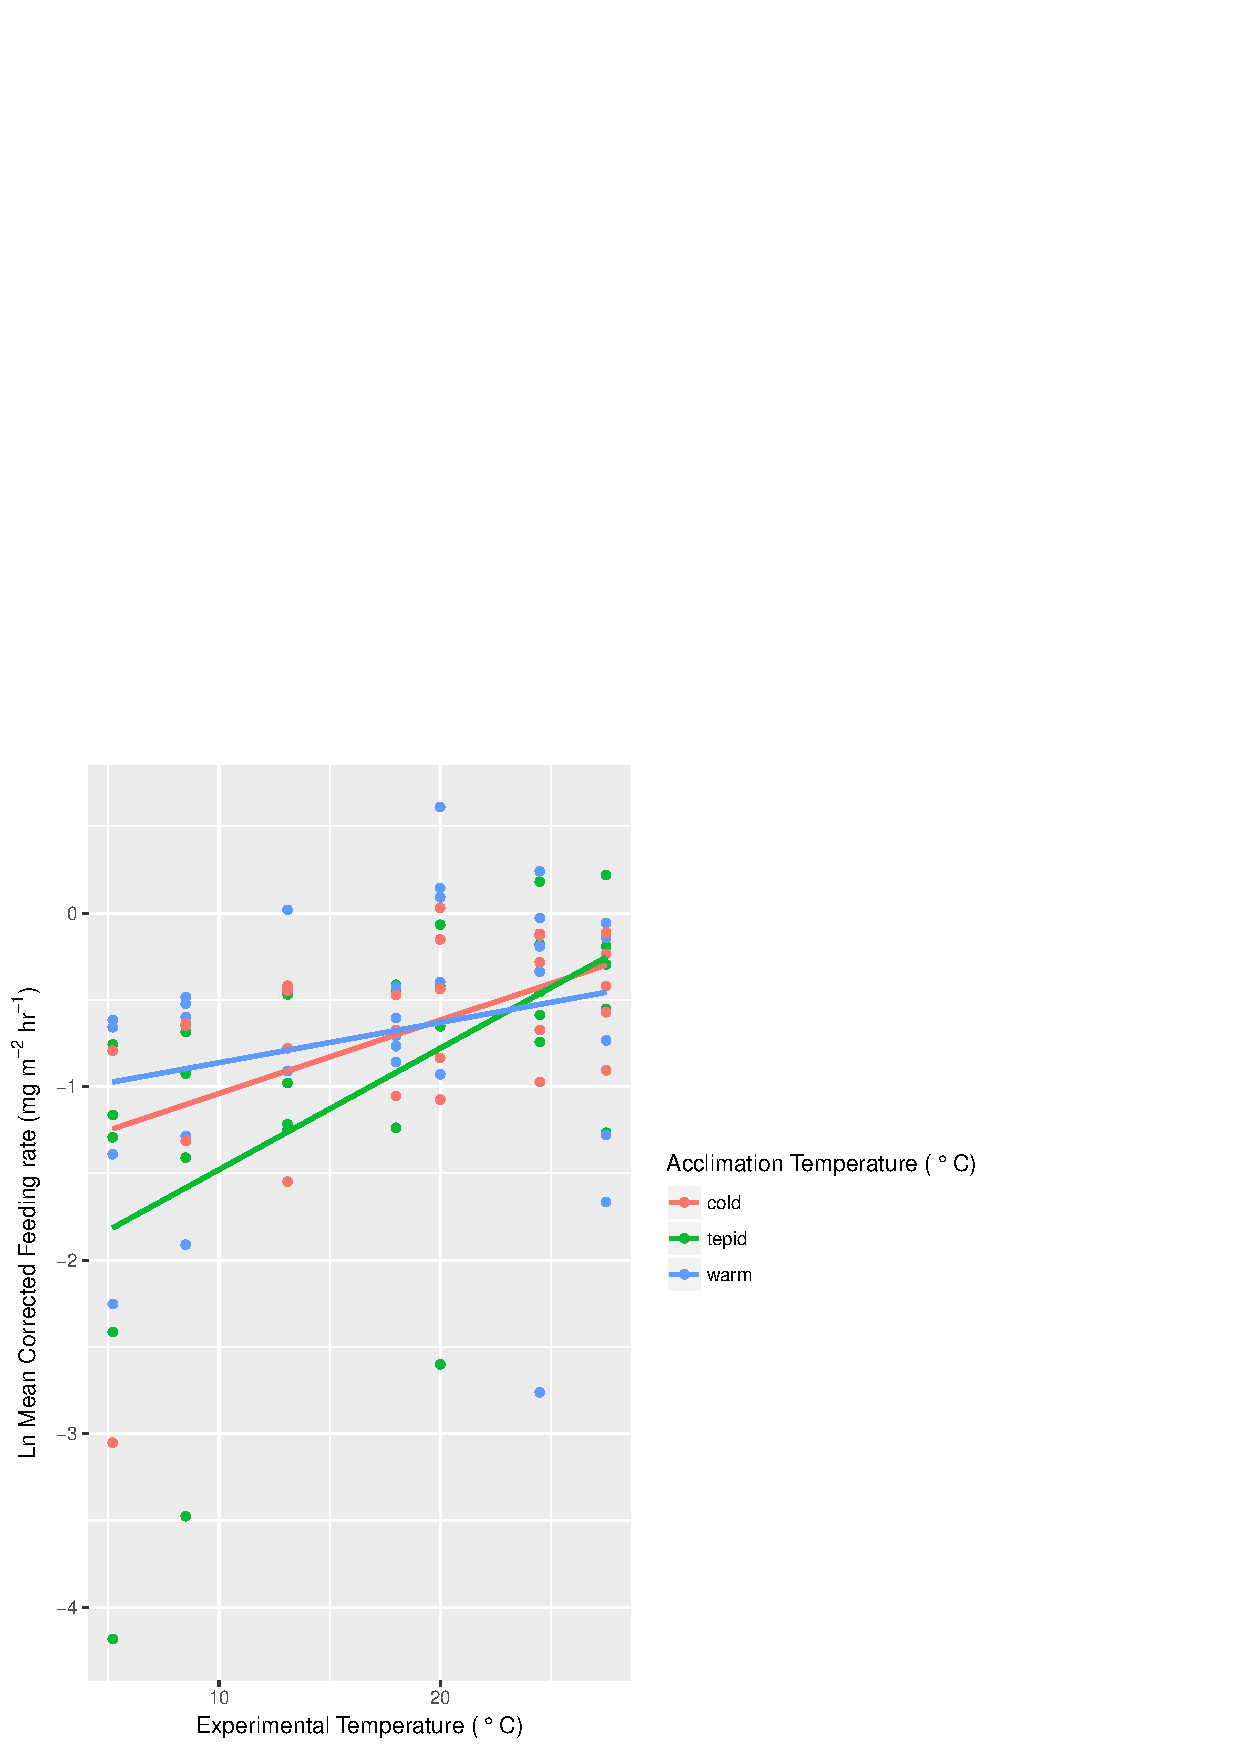
\includegraphics{meancorrectedfeeding_vs_exp_acctemp.pdf}
\caption{Feeding rate response of \textit{R. balthica} to experimental temperature, with    
acclimation temperature included as a factor.}
\end{figure*}

\subsection*{Linear}

Linear models were plotted on all biological trait data using 
the following equation from the Metabolic Theory of Ecology 
(\cite{gillooly_effects_2001,savage_effects_2004}):

\begin{equation}
B = B_{\theta} e^{E_t\frac{T_t - T_0}{kT_tT_0}}
\end{equation}

Where B is the trait of interest, $B_0$ is the constant, $E_t$ is the 
activation energy of the trait, $T_t$ is the experimental temperature (5 - 
30\degree C), $T_0$ is the average of the experimental temperatures used (17.5\degree C) and k is the Boltzman constant. The equation was subsequently logged to allow for linear models to be plotted.


\begin{figure*}[!b]

\centering
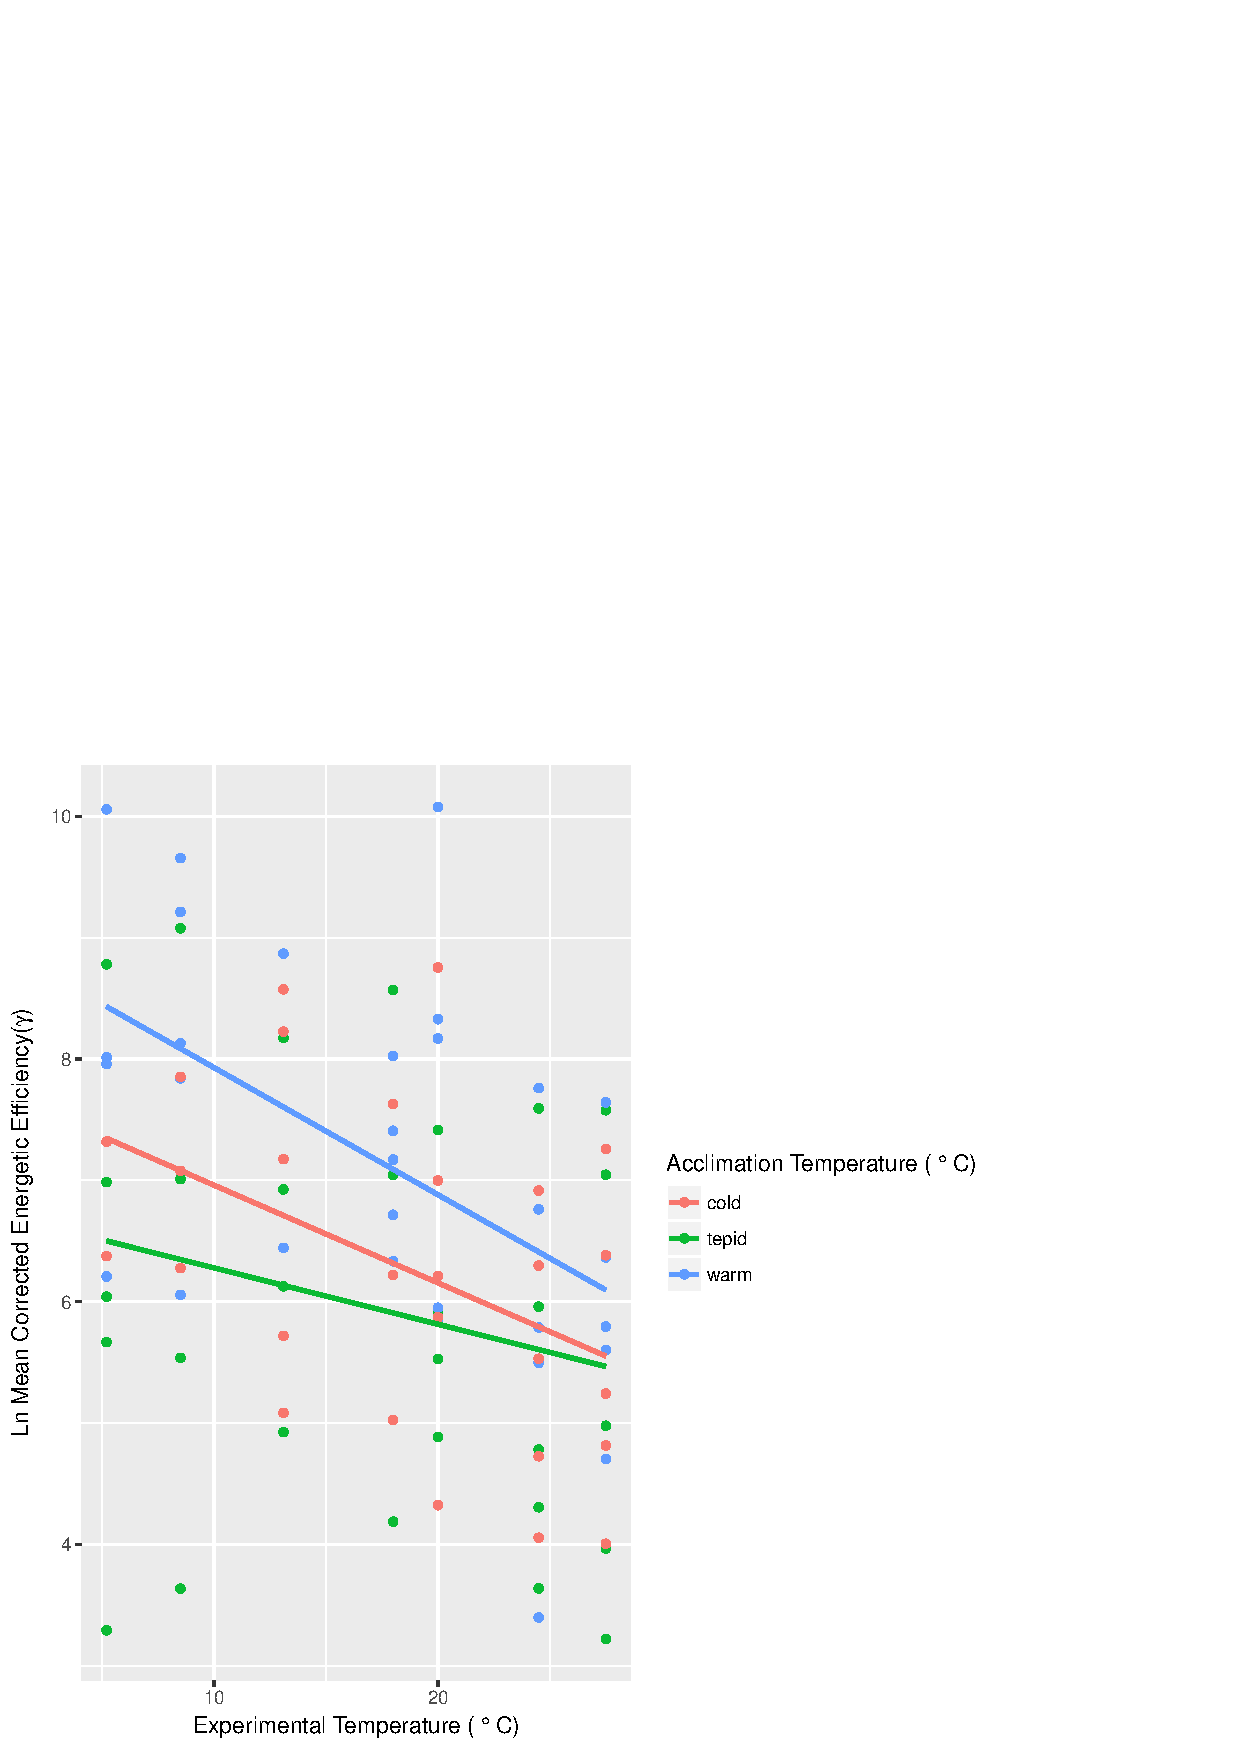
\includegraphics{meancorrectedeneff_vs_expacctemp.pdf}
\caption{Energetic efficiency response of \textit{R. balthica} to experimental temperature, with    
acclimation temperature included as a factor.}
\end{figure*}


\begin{figure*}[!t]
\centering
\includegraphics{meancorrectedeneff_vs_acctemp.pdf}
\caption{Energetic efficiency of \textit{R. balthica} plotted against acclimation temperature. Tepid (14.3\degree C) and
warm (19.3\degree C) acclimation differed significantly (p \textless 0.01), whilst cold (9.6\degree C)/warm
and cold/tepid returned non-significant results
( p \textgreater 0.08).}
\end{figure*}

\subsection*{Model comparison}

In order to compare the fits of models to
the respiration data, Akaike’s Information Criteria (AIC), Bayesian Information Criteria 
(BIC) and R$^2$ values were calculated. Both IC's have their 
merits, and so both were calculated to ensure the best fitting 
models were correctly identified. Models with lower AICs/BICs were considered 
to be better predictors of the data.

R$^2$ values show how well the model fits the data; the higher the R$^2$ value 
the more the model explains the data.



\subsection*{Statistical analysis}

All statistical analses were carried out in R version 3.2.3 (\cite{r_core_team_r:_2013}).
ANCOVAS (Analysis of Covariance) were used to explore relationships between the 
dependant variables (respiration rate, feeding rate or energetic efficiency) and Temperature, 
both acclimation and experimental. The experimental temperature was run in the
model as a continuous explanitory variable, while the acclimation temperature
was used as a categorical variable with the levels: cold, tepid and warm. 

















\end{document}